\section{Cenários}
\vspace*{1cm}
Antes mesmo de se apresentar os estudos de casos, é preciso explicar o que são estudos de caso.
Estudo de caso nada mais é que uma pesquisa que visa ser modelo de referência para aquilo que será proposto. Ao mudarmos a frase “Nada se cria, tudo de cópia” para, “Nada se cria, tudo se referência”, conseguimos entender que para se criar algo diferente, foi necessário uma mínima referência que seja, com isso surge os estudos de caso, que ajudam a buscar referências em aspectos diferentes em diversas situações.

\subsection{Console}


\subsubsection{Estudo de caso - Gestão empresarial}

Na parte console o aplicativo da FoF visa facilitar e ajudar o cadastro de funcionários em massa de empresas que são parceiras, então porque não utilizar como referência softwares que gerenciam estoques, com entrada e saída em massa de dados. Mesmo assim esse nicho é enorme, o filtro necessita ser maior, para uma melhor compreensão e fácil entendimento para a realização dos estudos baseados no cadastro em massa.

Após pesquisas, chegamos nos sistemas ERP ( Enterprise Resource Planning, ou em português Planejamento dos Recursos da Empresa ), com isso a busca fica mais linear em um objetivo que consegue abranger muitos pontos.

\begin{figure}[!h]
	\centering
	\caption{Representação gráfica de ERP}
	
\includegraphics[width=200px, height=200px]{./images/erp.png}
	\par{Autor(a): Desconhecido}
\end{figure}

Exemplo básico de como se funciona sistemas ERP com módulos acoplados, que podem fazer ele ser completo, criar um sistema utilizando essa base nos traria mobilidade e abriria um grande espaço para podermos esculpir o sistema da nossa maneira sem esquecer da essência de um sistema ERP.

Com todo esse conhecimento adquirido, e a ideia formada, foram "buscados" no mercado tipos de sistemas ou empresas que conseguiam suprir essa necessidade, de uma forma simples mas eficaz, e que sabiam trabalhar com sistemas ERP, e após pesquisas SGB foi a selecionada por conta do seu repertório. 

A SGB é uma empresa especializada em Sistemas de ERP de Gestão Empresarial, estando no mercado desde 2000 buscando inovar cada vez mais no mercado com seus produtos.

\begin{figure}[!h]
	\centering
	\caption{Auditoria de Produtos}
	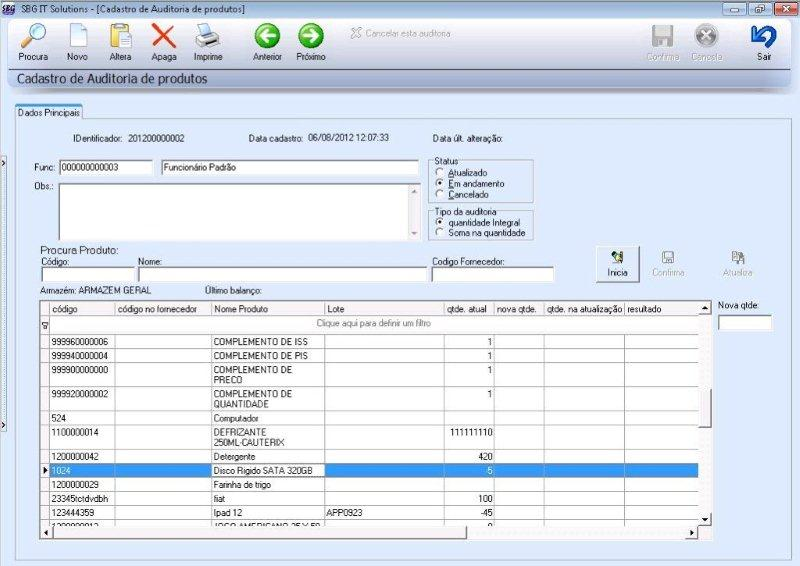
\includegraphics[width=300px, height=190px]{./images/SGB1.jpg}
	\par{Autor(a): \cite{sbg}}
\end{figure}

\begin{figure}[!h]
	\centering
	\caption{Cadastro de Produtos Avançados}
	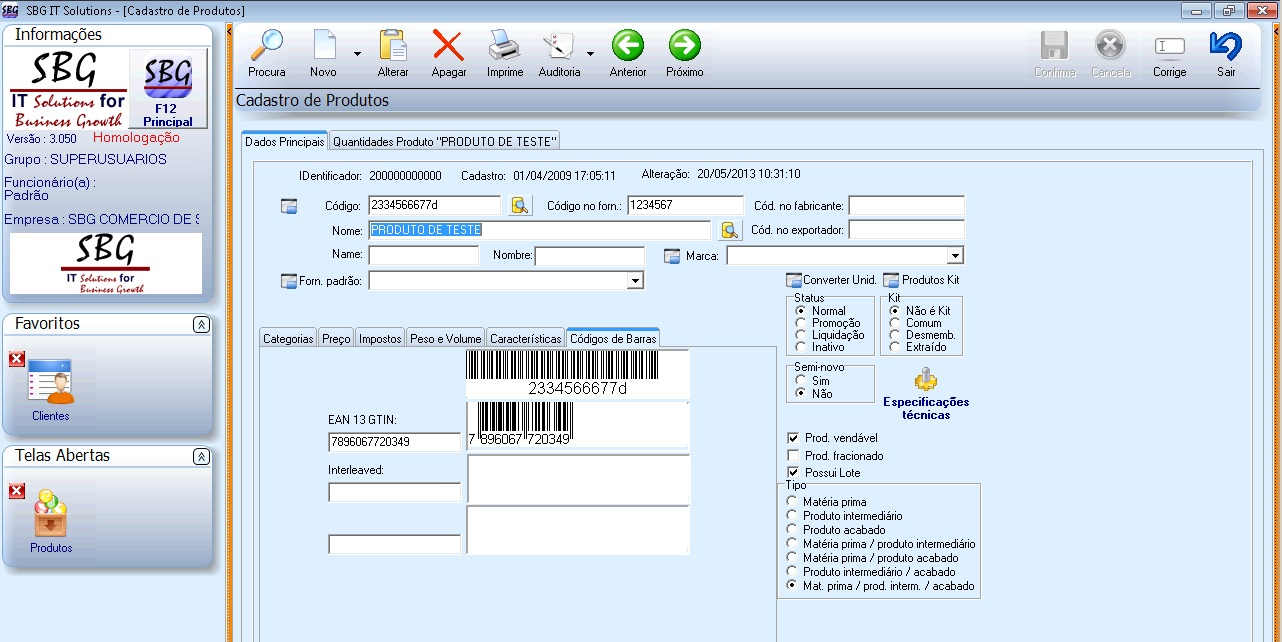
\includegraphics[width=300px, height=190px]{./images/SBG2.jpg}
	\par{Autor(a): \cite{sbg-1}}
\end{figure}
\newpage

Analisando a forma na qual as informações são cadastradas e compreendendo a maneira na qual esses sistemas trabalham, conseguiu-se chegar no primeiro protótipo de visualização e seleção de dados em massa da FoF, buscando trazer uma essência mais nova, mais simples porém completamente capaz de realizar suas funções e aberta a modulação.

\begin{figure}[!h]
	\centering
	\caption{Protótipo 1 da FoF}
	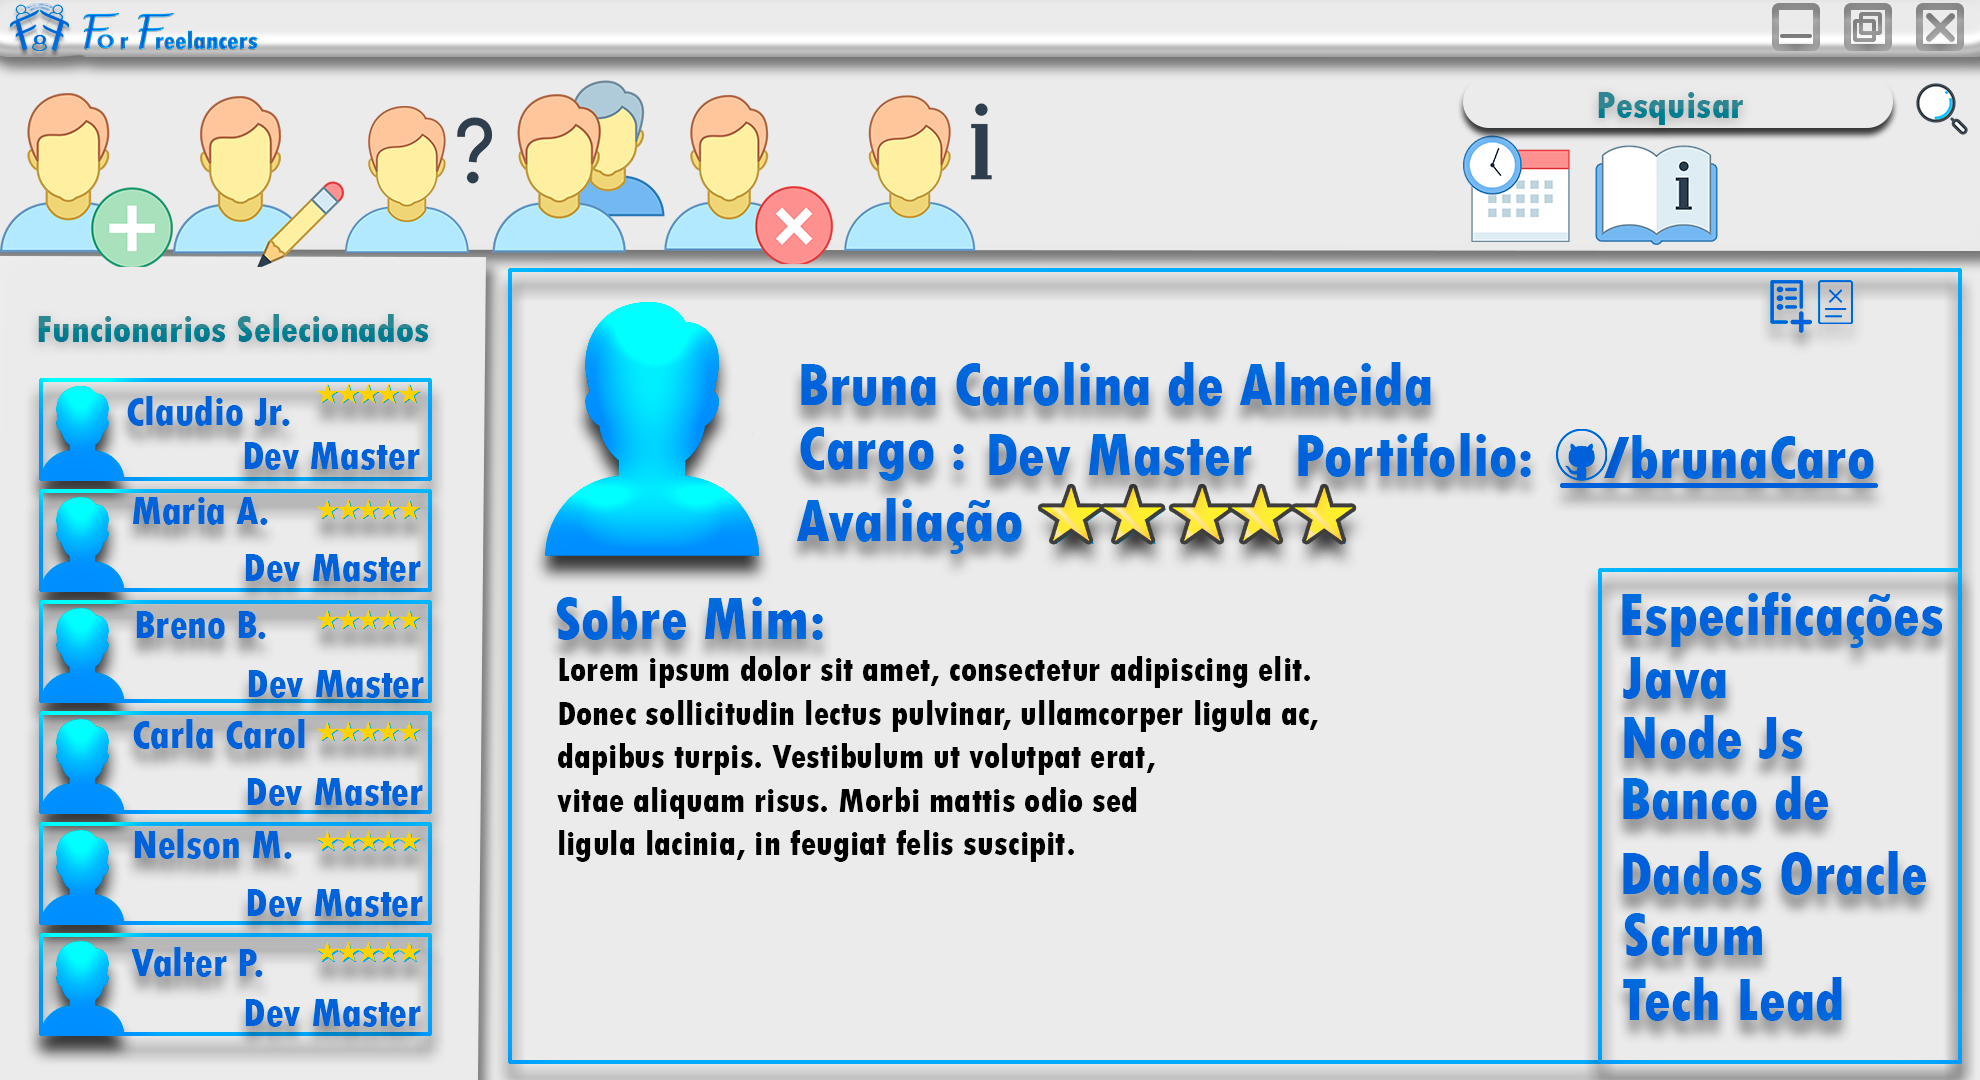
\includegraphics[width=400px, height=200px]{./images/prototipo1.png}
	\par{Autor(a): Hakawã Alves}
\end{figure}

\subsubsection{Estudo de caso - Modulação}

Como dito no tópico acima, a ideia de ter um sistema com uma fácil aceitação a novos módulos era o objetivo. Tendo isso como um primeiro norte, e sabendo que a FoF esta sempre buscando inovar no mercado, fazer um sistema que aceite módulos open source( Codigo fonte de utilização livre ), possibilitaria, à comunidade das empresas que utilizam nosso sistema, se unir e criar novos módulos independentes, podendo até mesmo reunir uma equipe para criar seu próprio módulo e distribuir com a comunidade. Obviamente que todo novo módulo criado passaria pela aprovação da FoF para ver se ele não é malicioso ou que busque quebrar dados sigilosos de outras empresas.

Muitas empresas utilizam sistemas modulares, afinal isso traz uma liberdade de comprar um software e os módulos que são necessários. No entanto, o difícil de se encontrar no mercado uma que tenha uma comunidade trabalhando em conjunto e criando seus próprios módulos para suprir suas necessidades. Isso levou a decisão de mudar um pouco a direção do olhar.

Utilizando como metáfora Simba e Mufasa (\citeyearpar{rei-leao}Rei Leão), sentados no monte, onde, Mufasa mostra ao filho o tamanho do reino com a frase “Tudo isso que o sol toca é nosso reino”, só estávamos olhando
aonde o “sol tocava”, que eram as empresas que utilizavam/criavam sistemas modulares. Para buscar   
novas possibilidades ficamos interessados igual ao Simba quando pergunta para seu pai “E aquele lugar escuro lá”, sendo que o lugar escuro no filme é um lugar além do reino, um lugar onde Mufasa não tem domínio, mas na nossa realidade aquele lugar escuro era a comunidade de games, especialmente a comunidade do Nexus Mod de Skyrim.

\begin{figure}[!h]
	\centering
	\caption{Mufasa e Simba}
	
\includegraphics[width=400px, height=200px]{./images/mufasa.jpg}
	\par{Autor(a): The Walt Disney Company}
\end{figure}

Nexus Mod é um gerenciador de Mods(Modulações/Modificações) para games. Eles abrangem inúmeros jogos, mas a categoria de Skyrim( Jogo desenvolvido pela Bethesda, lançado em 2011) foi a escolhida como referência, pois a maneira que essa comunidade trabalha é especial. Cada novo dia, semana nova, mês novo, surgem novos mods no qual a experiência do jogo é modificiada, revivendo-o de uma nova maneira, fazendo isso ele entra em um ciclo renovável. 
É isso que a FoF busca em seu sistema, construir uma comunidade na qual a mesma ajude a manter o ciclo de vida do sistema renovável e inovador a cada dia que passa. 

\begin{figure}[!h]
	\centering
	\caption{Nexus Mod versão web na categoria 30 dias}
	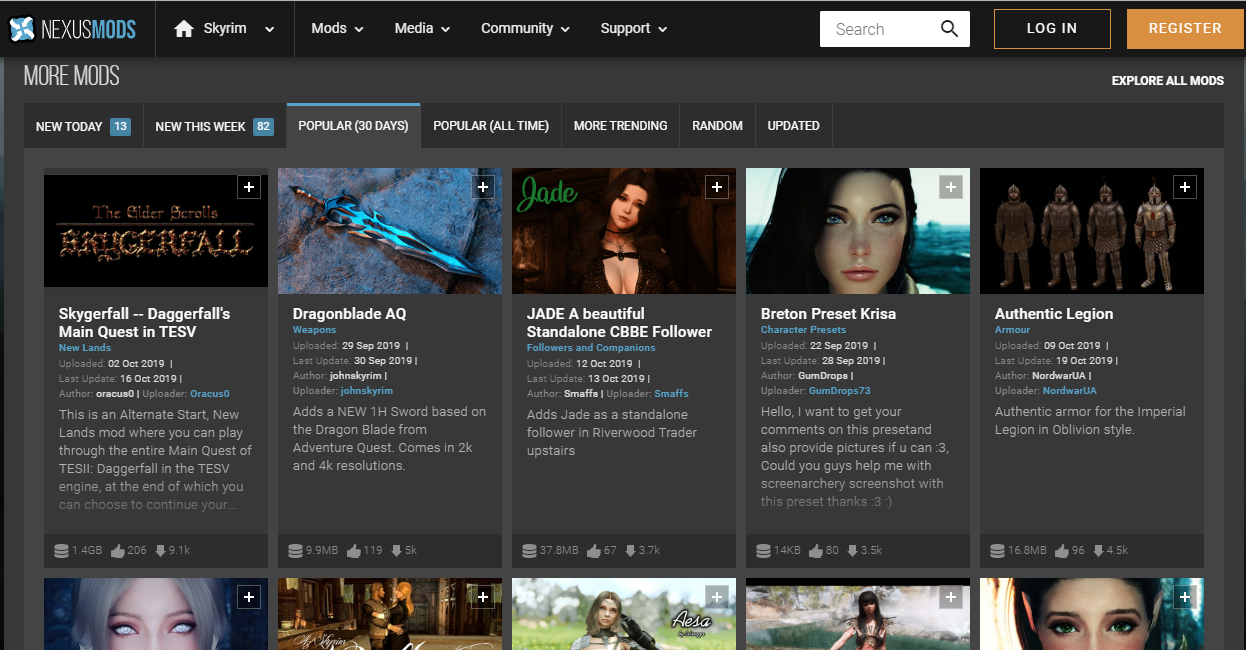
\includegraphics[width=300px, height=120px]{./images/nexusMod.png}
	\par{Autor(a): \cite{nexus-mod}}
\end{figure}

\begin{figure}[!h]
	\centering
	\caption{Nexus Mod Manager }
	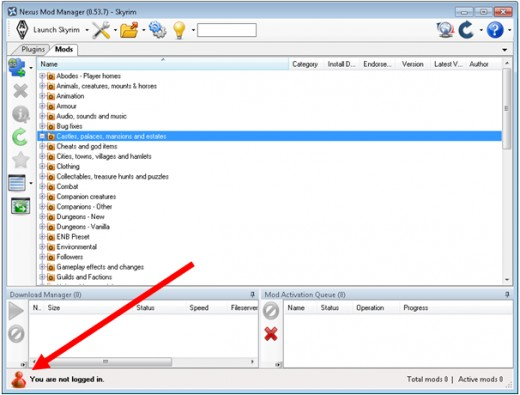
\includegraphics[width=300px, height=140px]{./images/nexusMod3.jpg}
	\par{Autor(a): \cite{nexus-mod}}
\end{figure}

\newpage

\subsubsection{Estudo de caso - Informações em massa}

Gestão empresarial e modulações são alicerces que queremos erguer para conseguirmos dar total suporte as plataformas web e mobile. Uma empresa conseguiria cadastrar inúmeras vagas de freelas de maneira rápida utilizando nosso sistema console, de forma que todas essas informações sejam disparadas automaticamente para nossas plataformas, permitindo uma maior velocidade/agilidade na qual esses dados são compartilhados.

Além de até mesmo poder permitir o uso de uma nova modulação, que ajude a selecionar todos os candidatos de uma X categoria e enviar mensagem para eles automaticamente dizendo que todos passaram de fase, e que a segunda fase acontecerá na quinta-feira por exemplo, é uma maneira de facilitar a comunicação e transação de informações.

Vendo o momento atual de nosso país muito se fala na CPI da FakeNews( CPI - Comissão parlamentar de inquérito, FakeNews – Notícias falsas), que houve inúmeros disparos de vários candidatos espalhando notícias falsas, pagando empresas com dinheiro público para realizar esses ataques uns contra os outros via whatsapp.

Apesar de ter sido usado de forma errada, de maneira maligna, isso nos deu uma ideia de como funcionaria esses disparos de informações. Da mesma maneira que se foi realizada a busca no mercado atrás de uma empresa que fosse especialista em sistemas ERP, agora voltado ao nicho de disparo de informações, encontramos a Housoft (Uma empresa especializada em disparo de dados em massa), a qual tem uma interface e um funcionamento simples, o que facilitou compreender como iriamos realizar a distribuição das informações enviadas pelas empresas para popularizar as outras plataformas.

\begin{figure}[!h]
	\centering
	\caption{Housoft lobby de entrada do sistema}
	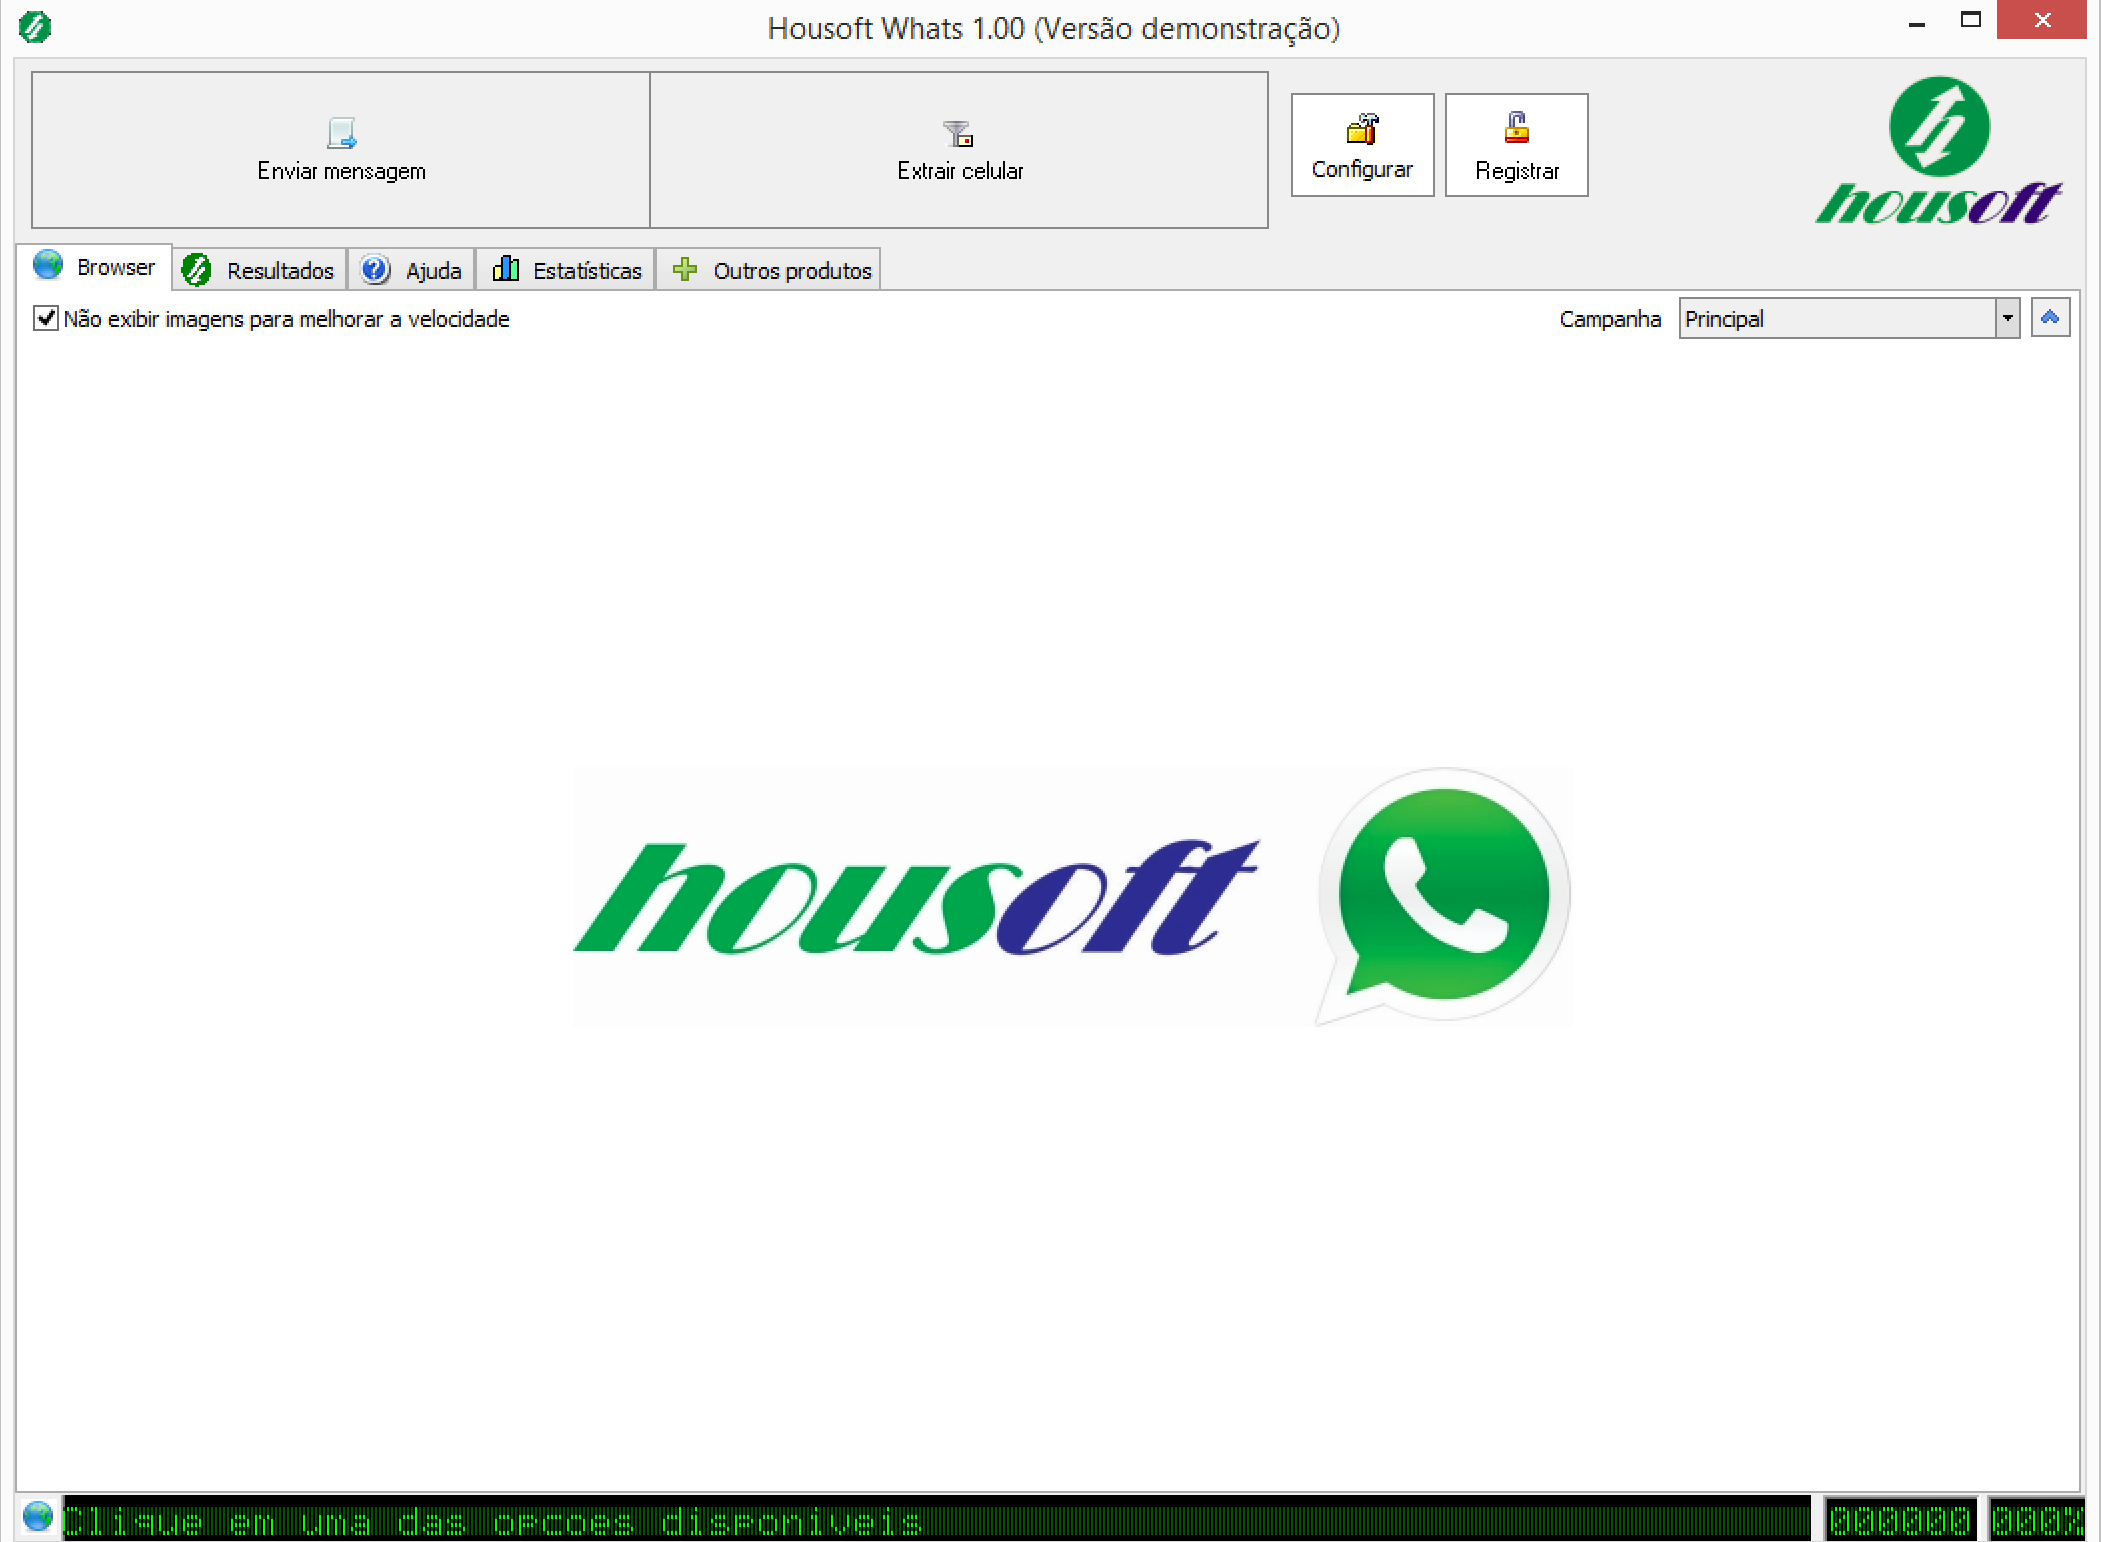
\includegraphics[width=400px, height=200px]{./images/housoft.png}
	\par {Autor(a): \cite{housoft}}
\end{figure}

\begin{figure}[!h]
	\centering
	\caption{Configuração para disparar pedidos de amizade no facebook}
	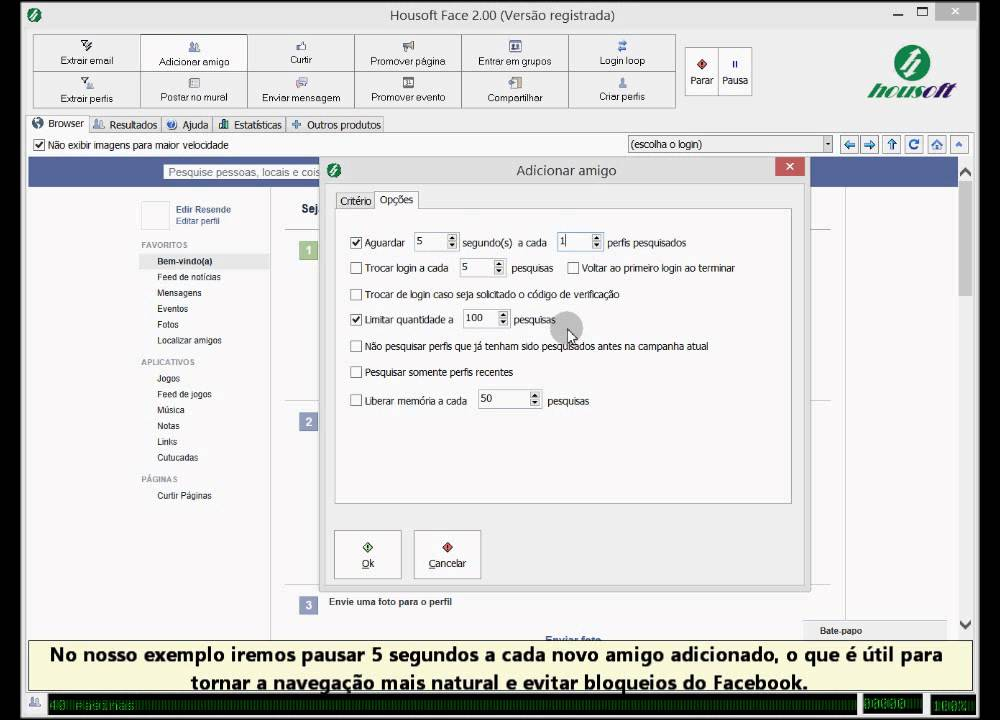
\includegraphics[width=400px, height=200px]{./images/housoft1.jpg}
	\par {Autor(a): \cite{housoft}}
\end{figure}

\newpage

\subsection{Plataforma Web}

\subsubsection{Estudo de Caso - LinkedIn}

O LinkedIn é uma plataforma web com formato de rede social voltada para o mercado de trabalho, onde os usuários podem compartilhar seus conhecimentos, experiências, divulgar atividades profissionais, voluntariado, pesquisas e entre outros. 

Ele teve sua ideia introduzida em 2002 e começou dentro de uma sala de estar nos Mountain View, Califórnia, EUA pelo Reid Hoffman co-fundador, sendo que além de Hoffman outros também fazem parte da fundação, como Allen Blue, Konstantin Guericke, Eric Ly e Jean-Luc Vaillant. Suas atividades como empresa começaram a partir de 2003, no dia 05 de Maio, quando os fundadores convidaram seus antigos colegas para serem os primeiros membros da rede social.

No decorrer dos anos e com o crescimento dos membros, novas ferramentas eram necessárias para os usuários, dentre elas vale destacar algumas, sendo elas mencionadas nos próximos parágrafos.

Em 2004 uma nova ferramenta foi introduzida capaz de adicionar endereços e também de criar grupos voltada para temas específicos. No mesmo ano sendo feita uma parceria de grande credibilidade para a página, a American Express, dando ao LinkedIn um novo passo e também divulgação da plataforma. 

Em 2005 e 2006 foram introduzidas novas ferramentas, que até hoje são destaques na plataforma, “Jobs and Subscriptions” (Empregos e Assinaturas), “Pessoas em sua rede social e torna-se exponencialmente com grande capacidade de crescimento. Já em 2007 oferecem novas linguagem para a plataforma como espanhol e francês.

Em 2009 Jeff Weiner passa a ser o novo CEO (Diretor Executivo) e presidente do LinkedIn, nesse período entre 2009 e 2011 foram os anos de maior crescimento da plataforma. Detalhe que em 2010 o LinkedIn foi lançado em Português e teve seu primeiro escritório no Brasil no ano de 2011, neste mesmo ano, a rede social atinge 90 milhões de usuários e entra, pela primeira vez, na bolsa de valores.

Em 2016, a Microsoft comprou o LinkedIn por cerca de US\$ 26 bilhões e em 2017 a plataforma foi registrada com mais de 500 milhões de membros em mais de 200 países.

\begin{figure}[!h]
	\centering
	\caption{Pagina de perfil do usuário }
	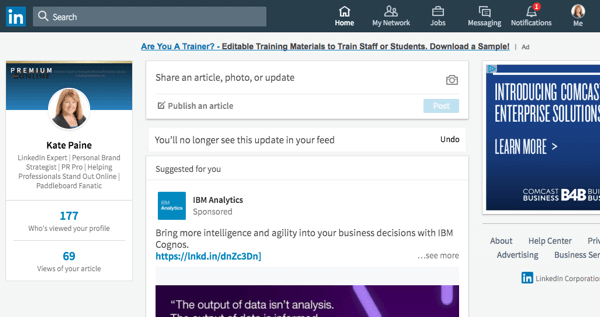
\includegraphics[width=400px, height=200px]{./images/linkedin1.png}
	\par {Autor(a): \cite{linkedin}}
\end{figure}

\newpage

Exemplo de perfil da plataforma LinkedIn, sendo semelhante a um currículo, onde o usuário pode listar suas habilidades, conceber resumos das atividades profissionais, exibir sua vida acadêmica e histórico de trabalho.
 
A plataforma conta hoje com grandes melhorias desde o começo, graças ao avanço das tecnologias e também da empresa que acompanhou as mudanças e tornando-se a plataforma principal em divulgação de vagas de trabalho e recrutamento. 

Algumas funções tem o papel importante na plataforma. Pode-se destacar algumas funções como:

Sendo acessada no menu principal o \textbf{\emph{Chat box}}(Mensagens): É importante para a comunicação entre os usuários, como exemplo, uma conversa de um gestor com um candidato para um determinado projeto ou trabalho.

No canto superior pode acessar em um ícone com o nome \textbf{\emph{Vagas}}: Nesse ícone é onde se encontram todas as vagas disponíveis, nas quais as empresas divulgam com todos os detalhes do perfil desejado, onde o usuário poderá ver no perfil da vaga se tem os requisitos necessários para prosseguir com a candidatura. 

Também no canto superior pode acessar um ícone chamado \textbf{\emph{Notificações}}: Esta função é para notificar o usuário das atividades ocorridas no tempo em que ele não estava online, mostrando quem curtiu sua publicação, vagas novas, quem enviou uma mensagem, qual curso está disponível e outras atividades.

Nas soluções do Linkedin, que são encontradas no canto superior direito descritas como Soluções, encontram-se algumas dessas que são destaque, como exemplo:

\textbf{\emph{Anunciar Vaga}}: Essa ferramenta é voltada para as empresas divulgarem suas vagas, sendo por meio desta ferramenta que ela é inserida no Vagas, para os usuários se candidatarem e de forma que os recrutadores possam analisar os perfis. 

\textbf{\emph{Profinder}}(Espaço para dedicado para projetos): Essa é uma ferramenta voltada para divulgação dos projetos já realizados, dos quais se destacam e ficam em evidência em um mural. Mas pode-se encontrar por pesquisa e filtros, projetos que sejam de algo específico, onde os usuários criaram e divulgam para que empresas possam ver e saber como cada um trabalha.

\textbf{\emph{SlideShare}}(Compartilhar Slides com diversos temas): Essa ferramenta proporciona que o usuário faça, por meio de slides com todas as informações inseridas, apresentações de seus projetos, conhecimentos, e feitos que são relevantes, entre outros.

\subsubsection{Estudo de Caso - Catho}

A Catho é uma empresa brasileira pioneira de tecnologia voltada para o mercado de trabalho, com objetivo de fornecer seleção e recrutamentos para seus clientes, ajudando-os em sua carreira, assim exercendo uma grande notoriedade na sociedade.

De acordo com seu site oficial, a Catho conta com mais de 7 milhões de cadastros para a seleção, sendo 4 mil novos currículos por dia, além de conter a maior base de candidatos profissionais PcD (pessoas com deficiência) com laudos válidos, de forma que os mesmos podem assinar o serviço catho gratuitamente.

Sua marca foi fundada em 1977, por Thomas Case, sendo assim, a primeira empresa a implementar este segmento no Brasil, sendo que a princípio o site era somente para cadastros de currículo dos clientes.

Em seguida, contando com a avaliação de informações e corroboração de dados, o processo de recrutamento e seleção da empresa passou a evoluir, assim facilitando as contratações.

Mais tarde passou a oferecer testes online e programa de cursos presenciais, de mesmo modo passou a fornecer anúncio de currículo e vagas de empregos para os profissionais, adotando este modelo de negócios até hoje. Oferecendo também diversos produtos para os dois públicos, tanto para os profissionais em busca de emprego como para as empresas.

Assinantes têm acesso a alguns serviços exclusivos, os quais podem, por exemplo, garantir a veracidade de anúncios divulgados, através de uma verificação dos dados cadastrais das empresas anunciantes e de suas vagas.

Os profissionais procuram na Catho não só oportunidades de trabalho, como também uma realização profissional, o que acaba juntamente auxiliando no crescimento das empresas, tornando-as mais produtivas.

A seguir estão alguns exemplos do portal da Catho e suas funcionalidades, onde seus os usuário e clientes podem pesquisar por vagas, cargos e empresas desejadas.

Na página inicial podemos encontrar em seu canto superior direito a função de acesso ao perfil ou cadastro, um pouco mais abaixo também uma caixa específica para cadastro e pesquisa de vaga.

\begin{figure}[!h]
	\centering
	\caption{Página inicial Catho }
	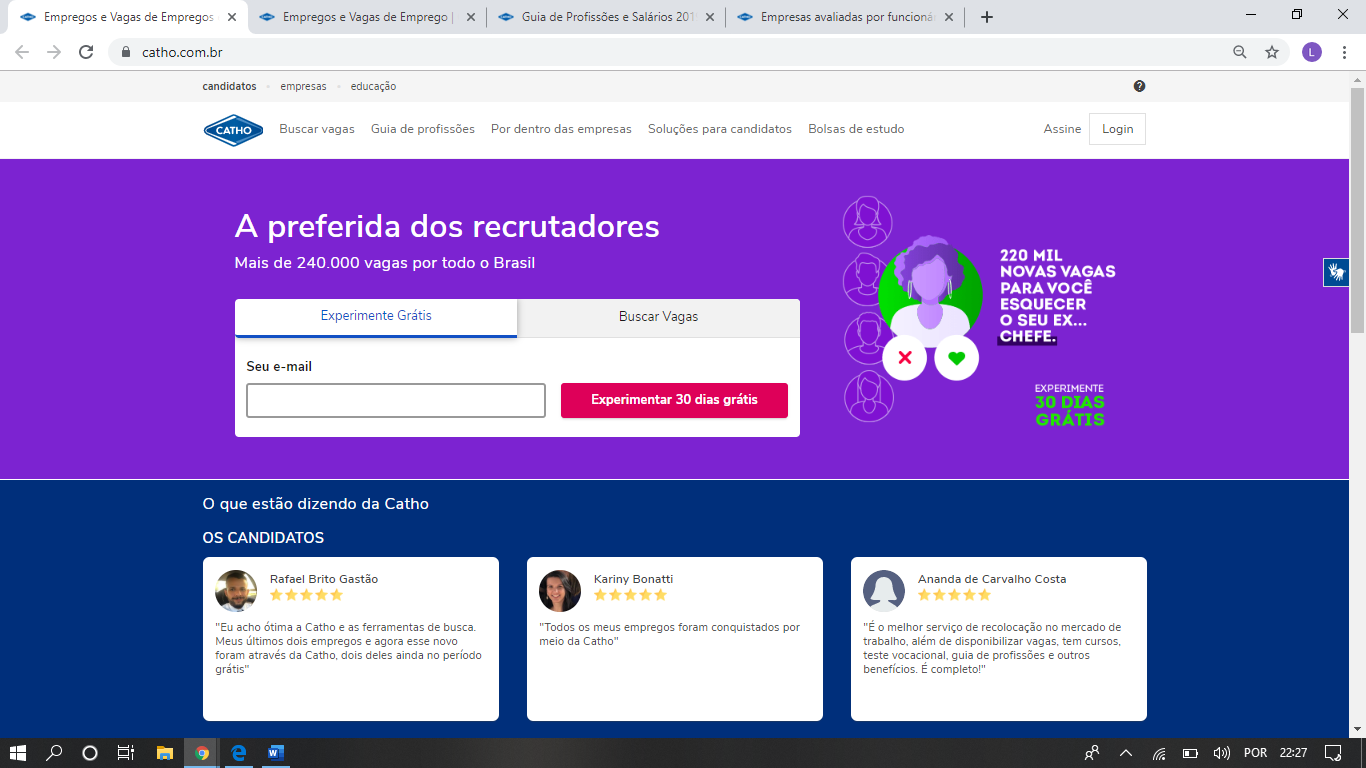
\includegraphics[width=340px, height=130px]{./images/cattho.png}
	\par {Autor(a): \cite{catho}}
\end{figure}
\newpage
Em sua barra de navegação, podemos observar outras funções tais elas como, buscar vagas, guia de profissões, e por dentro das empresas. Sendo que na primeira, podemos pesquisar propriamente por vagas filtradas por cargos, palavras chaves, região e salário desejado. Já na segunda, podemos pesquisar as vagas especificamente por cargos pretendidos. E por fim, na terceira, podemos escolher as vagas que as empresas oferecem.

A seguir tem-se imagens representando essas três funções:

\begin{figure}[!h]
	\centering
	\caption{Buscar vagas}
	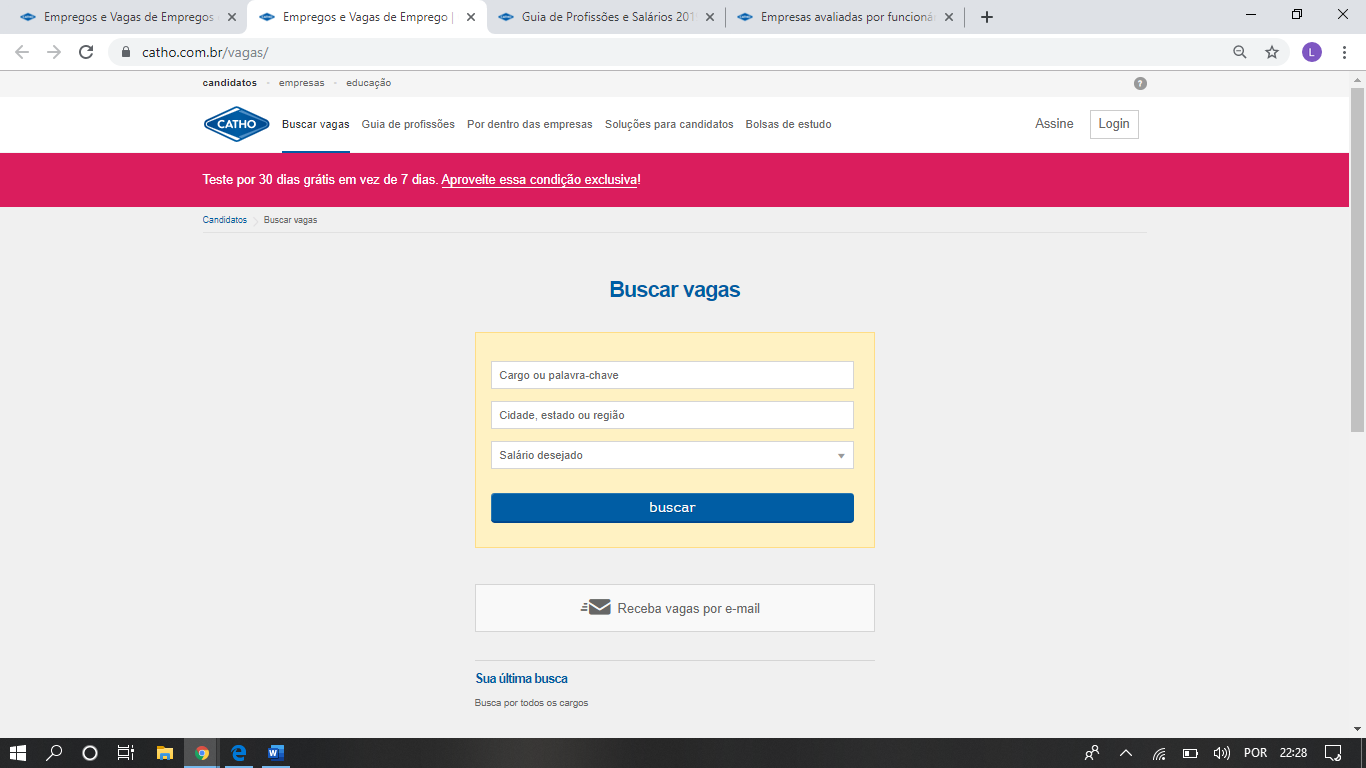
\includegraphics[width=380px, height=150px]{./images/cattho1.png}
	\par {Autor(a): \cite{catho-1}}
\end{figure}

\begin{figure}[!h]
	\centering
	\caption{Guia de profissões}
	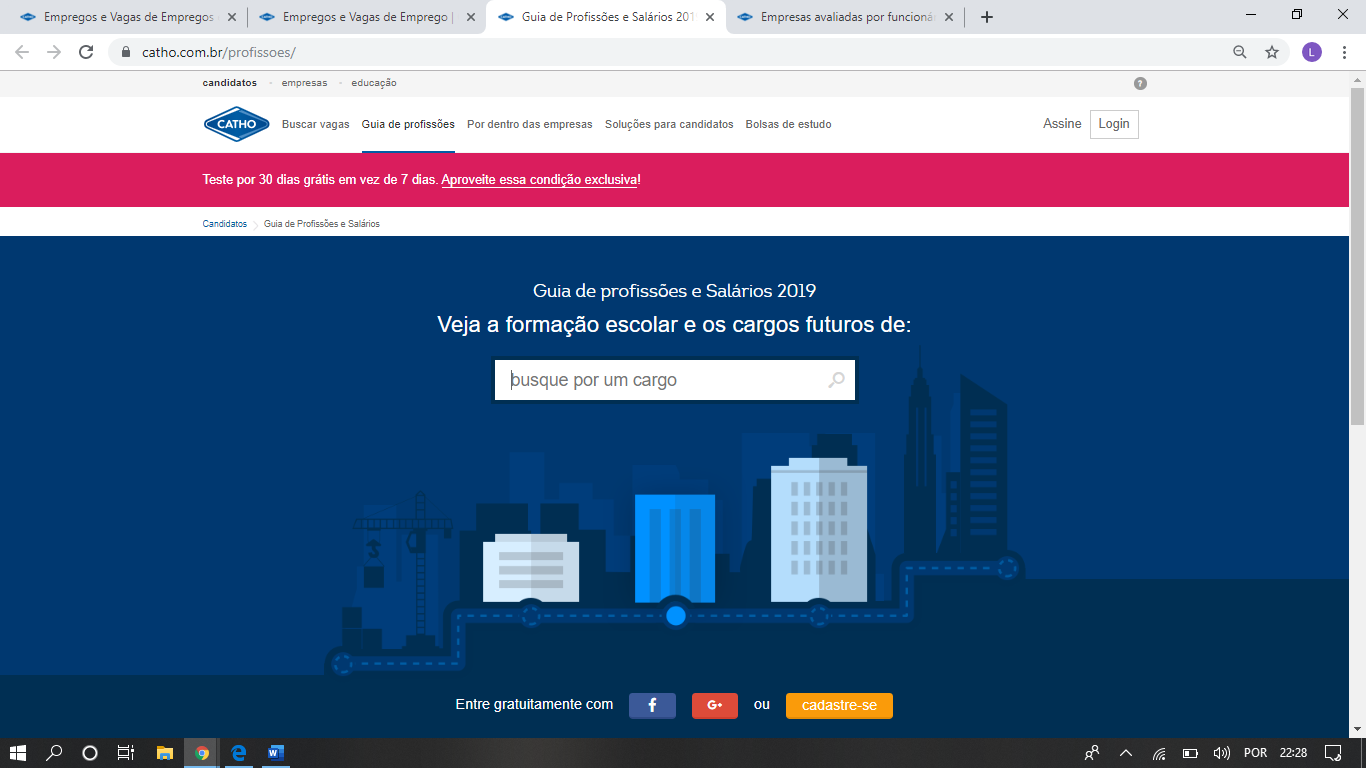
\includegraphics[width=380px, height=150px]{./images/cattho2.png}
	\par {Autor(a): \cite{catho-2}}
\end{figure}

\begin{figure}[!h]
	\centering
	\caption{Por dentro das empresas}
	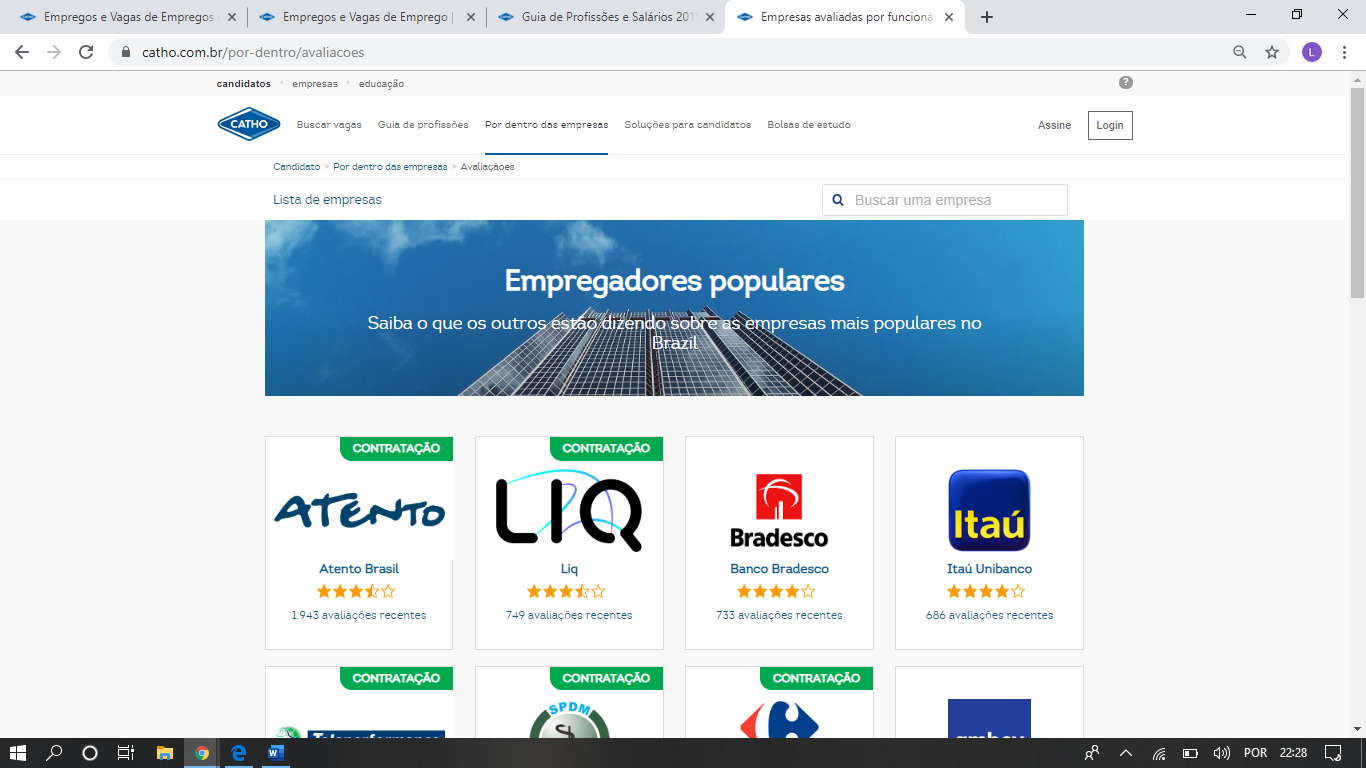
\includegraphics[width=380px, height=150px]{./images/cattho3.png}
	\par {Autor(a): \cite{catho-3}}
\end{figure}
\newpage 
\subsubsection{Estudo de Caso – GetNinjas}

Diferentemente dos outros dois estudos de casos da plataforma web, este foca na conexão entre profissionais e empresas, mas sim na disponibilização e procura de serviços, ou seja, na conexão entre alguém que esteja à procura de um serviço e um profissional que o ofereça.

O GetNinjas foi fundado por Eduardo L’Hotellier, CEO da empresa, em 2011 e é, assim como no caso anterior, brasileiro, sendo a maior plataforma de contratação de serviços do Brasil, estando disponível não só para web, como para Android e iOS também.

De acordo com informações coletadas de seu site, são mais de 500.000 profissionais cadastrados, 2.800.000 serviços contratados por ano, nas mais diversas áreas, 240.000 clientes satisfeitos com o serviço contratado através da plataforma por mês, e R\$450.000.000 por ano representando o valor que é embolsado por profissionais associados a ela.

Apesar de seu sucesso atualmente, como muitos, não foi de primeira que deu tudo certo. No começo os planos eram de se fazer todo o contato do cliente com o profissional de forma online, o que ocasionou no primeiro problema, o fato de não conseguir estipular o orçamento de forma correta e completar a transação, pois existem condições externas que vão além de apenas o serviço necessário, por exemplo o ambiente de uma reforma e seu entorno pode afetar a mesma de forma que o custo e esforço necessários variam. Assim, teve-se a primeira grande mudança, que foi a não restrição do processo ao contato completamente online.

Outro problema foi que nem sempre o profissional que o cliente escolhia estava disponível, até porque o contato era feito via e-mail, o que ocasionava em um atraso de dias, dependendo, na comunicação. Assim foram feitas adaptações para que o contato agora fosse feito via aplicativo, e que primeiramente fossem selecionados profissionais que se encaixam no perfil e os que se disponibilizassem seriam os que entrariam em contato com o cliente.

Assim, percebe-se que é através de tentativas e erros que se vai que o projeto vai se construindo, pois é praticamente impossível tudo acontecer perfeitamente de primeira.

Falando de como ela funciona, nesta plataforma os profissionais podem se cadastrar e oferecer seus serviços, e o cliente pode procurá-los de acordo com suas necessidades. De acordo com o que o cliente precisar serão apresentados três profissionais por perto que atendem ao que foi pedido e seu orçamento, e por fim o cliente escolhe qual melhor se adaptar ao que ele queria.

\begin{figure}[!h]
	\centering
	\caption{Home do site}
	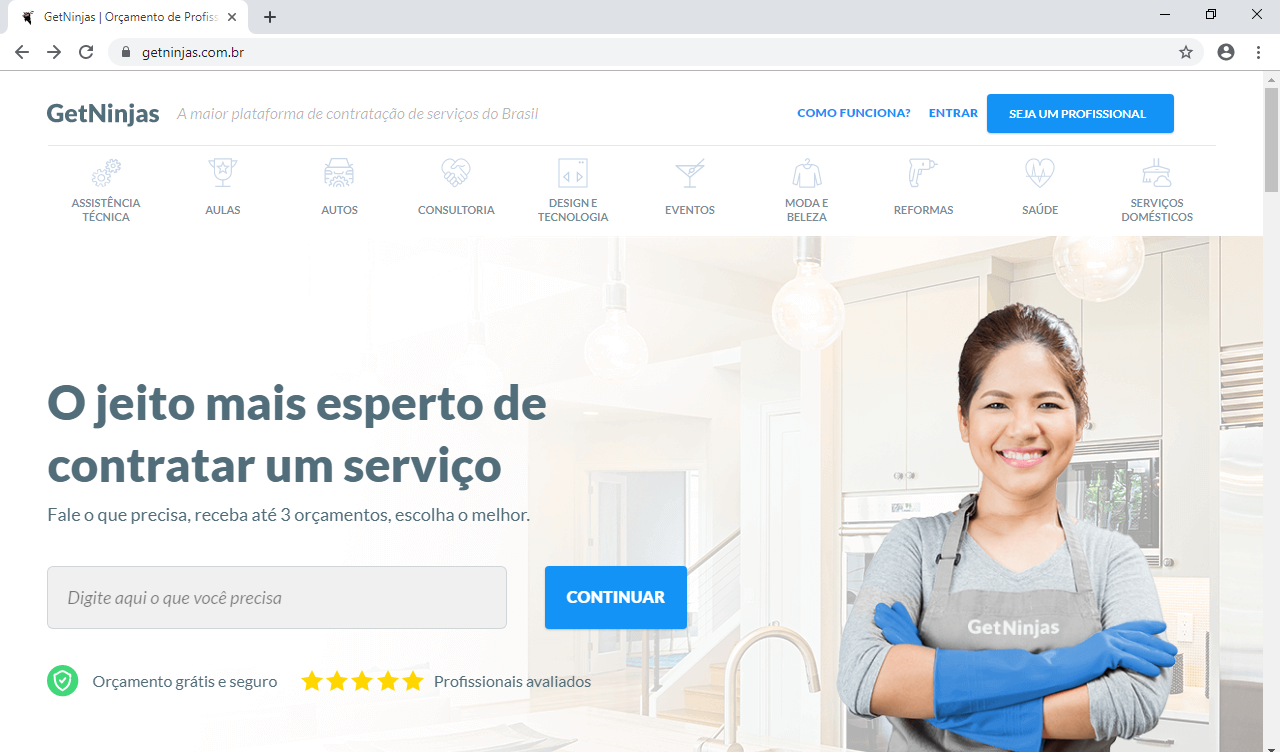
\includegraphics[width=390px, height=190px]{./images/getninjas.png}
	\par {Autor(a): \cite{get-ninjas}}
\end{figure}

Os serviços oferecidos são separados em dez áreas, de forma a facilitar a procura. São elas: assistência técnica, aulas, autos, saúde, consultoria, design e tecnologia, eventos, moda e beleza, reformas, saúde, e serviços domésticos. Sendo que, cada uma das áreas tem subcategorias.

\begin{figure}[!h]
	\centering
	\caption{Home do site com o menu de navegação aberto}
	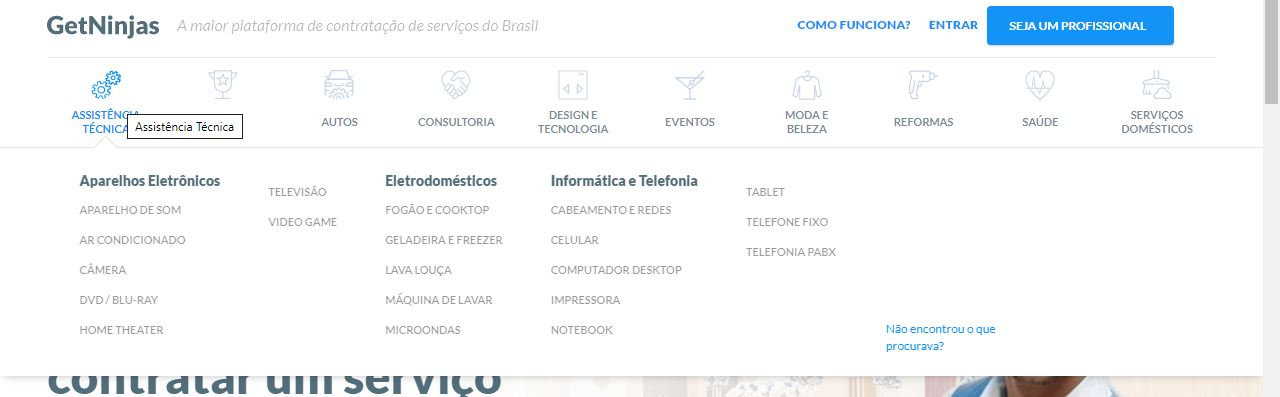
\includegraphics[width=320px, height=120px]{./images/getninjas2.png}
	\par {Autor(a): \cite{get-ninjas}}
\end{figure}


Apesar de ser uma plataforma gratuita, é necessário o uso de moedas internas para liberar o contato dos profissionais, mas sem garantia de que a transação será feita com sucesso após o contato, pois a plataforma permite o contato entre o cliente e o profissional, mas não é responsável pela transação em si. Da mesma forma, para que um profissional acesso os dados de seu cliente potencial ele precisa desbloquear usando moedas internas, as quais são vendidas em pacotes de diferentes valores para diferentes quantidades.


\begin{figure}[!h]
	\centering
	\caption{Anúncios e parcerias }
	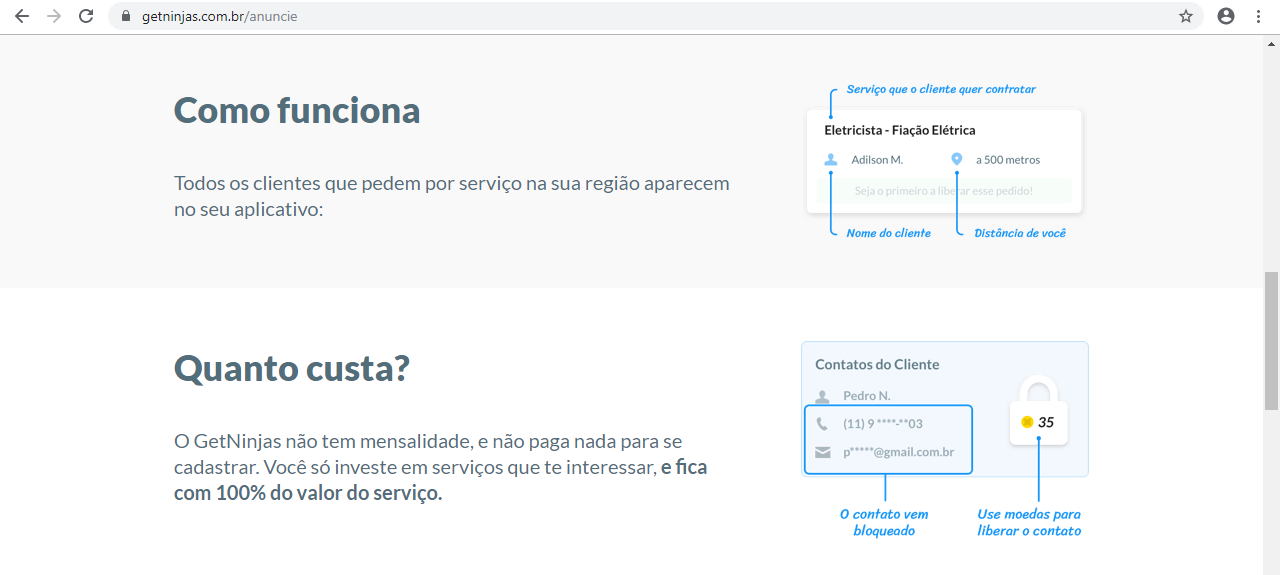
\includegraphics[width=400px, height=200px]{./images/getninjas3.png}
	\par {Autor(a): \cite{get-ninjas-a}}
\end{figure}


\subsection{Mobile}


\subsubsection{Estudo de caso - LinkedIn}

O LinkedIn é uma rede social feita para o meio profissional, ou seja, é destinada a pessoas que querem disponibilizar um perfil profissional para que outras pessoas possam visualizá-lo e assim ter conhecimento sobre seus dados, focados no meio corporativo.

É possível ter acesso ao LinkedIn de duas plataformas, web e mobile. O aplicativo mobile possui as mesmas funções da plataforma web, tendo em vista que o aplicativo mobile possibilita a utilização da rede social de qualquer lugar a qualquer momento, requerendo apenas uma conexão com a internet. Isto o diferencia de sua versão na plataforma web, que disponibiliza maior comodidade ao usuário, com a possibilidade de acessá-lo através de um computador. 

\begin{figure}[!h]
	\centering
	\caption{Interface mobile LinkedIn}
	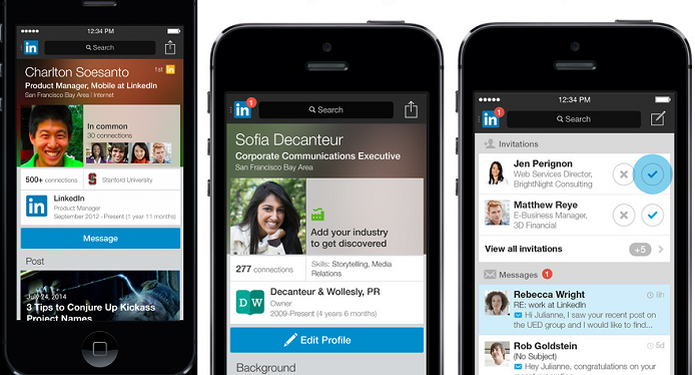
\includegraphics[width=300px, height=150px]{./images/linkedinMobile.png}
	\par {Autor(a): \cite{linkedin-b}}
\end{figure}
\newpage
A plataforma do LinkedIn possui algumas funções principais, sendo elas: disponibilizar uma lista de contatos, para assim o usuário sempre que precisar conseguir contatar alguma pessoa especifica; existe também a possibilidade de encontrar pessoas através dos contatos existentes; disponibilizar informações profissionais de modo que qualquer outro usuário possa facilmente encontrar um perfil com características específicas.

Outras funções também bastante relevantes seriam: buscar empresas que estejam disponibilizando vagas de emprego e, tendo em vista que como o usuário já possui em seu perfil as suas informações profissionais, é muito mais prático para a empresa, onde menos tempo será gasto, como por exemplo, solicitando informações; olhando do lado das empresas, as mesmas possuem a possibilidade de publicar vagas, para que outros usuários possam se cadastrar, e também podem criar publicações de assuntos profissionais.

\begin{figure}[!h]
	\centering
	\caption{Número de usuários do LinkedIn de 2009 até 2016 }
	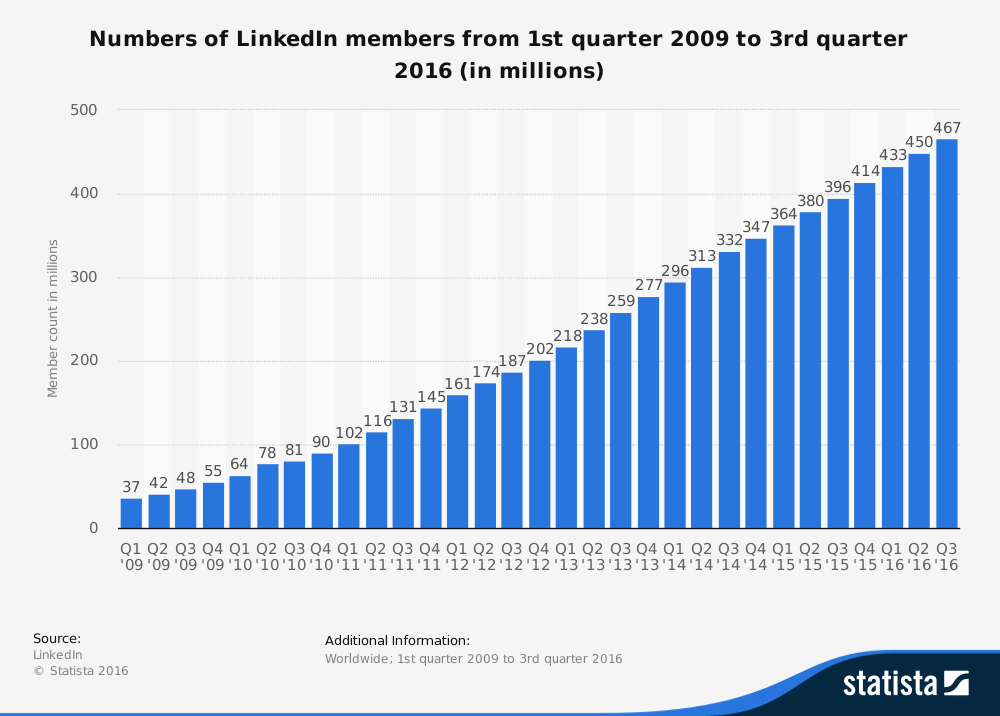
\includegraphics[width=300px, height=190px]{./images/linkedinMobile2.png}
	\par {Autor(a): \cite{linkedin-c}}
\end{figure}

A rede social fez muito sucesso, e é amplamente usado pela população, possuindo a incrível quantidade de mais de 500 milhões de usuários. Muitas oportunidades de emprego foram geradas através da plataforma, fazendo assim com que a taxa de desemprego diminuísse e gerando lucro para as empresas.


\subsubsection{Estudo de Caso – Catho}

Como mencionado anteriormente, a Catho é uma plataforma com foco principal em empregabilidade, ou seja, ela disponibiliza ferramentas para auxiliar a busca por vagar de emprego para usuários, e possibilita publicação de vagas de emprego para empresas.

A plataforma é bem completa, contando com um aplicativo mobile para ser acessado facilmente por qualquer smartphone que tenha acesso à internet, além de estar disponível no ambiente web, podendo ser acessado pelo browser de qualquer computador ou aparelho que consiga ter acesso a um browser.

A plataforma mobile disponibiliza praticamente as mesmas ferramentas e funcionalidades que a plataforma web, dentre as quais pode-se destacar algumas: como já citado anteriormente, a plataforma conta a funcionalidade principal de possibilitar que empresas possam divulgar vagas de emprego e usuários possam se candidatar a essas vagas; é possível também disponibilizar um currículo em um perfil no Catho, para que assim as empresas tenham a facilidade de visualizar as informações profissionais do usuário; um guia de profissões está disponível na plataforma, para que os usuários possam ter uma orientação sobre como funcionam as profissões, para auxiliar na escolha da profissão que mais está de acordo com o perfil profissional dos mesmos.

Ela também apresenta uma área com informações sobre as empresas, nesta área é possível conhecer um pouco mais sobre as empresas cadastradas na plataforma, além de também possibilitar que os usuários possam avaliar as empresas. Outra função interessante é a de poder encontrar bolsas de estudo, sendo disponibilizadas diversas delas na plataforma, fazendo assim com que os usuários possam ter a oportunidade de adquirirem alguma formação, capacitando-os para o mercado de trabalho.


\begin{figure}[!h]
	\centering
	\caption{Interface mobile Catho}
	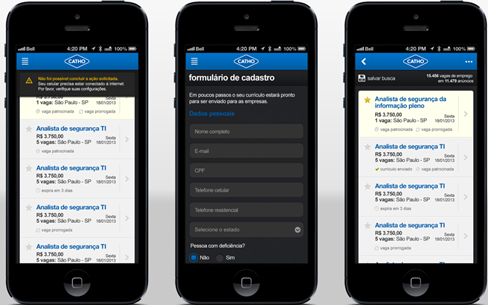
\includegraphics[width=350px, height=190px]{./images/cathoMobile.png}
	\par {Autor(a): \cite{catho}}
\end{figure}

\newpage

Contudo, a plataforma não é gratuita, contando com diversos planos de assinatura, com preços que variam de R\$ 26,00 à R\$ 134,00. Cada plano tem suas peculiaridades, como por exemplo: os planos mais caros possuem à análise do currículo do usuário, uma clara vantagem para as pessoas que não sabem bem como elaborar um currículo. Porém, por um período de 30 dias, a plataforma é gratuita para ser usada. Após este período é necessário que algum dos planos seja adquirido.

Gerando diversas vagas de emprego para seus usuários, a Catho faz um grande sucesso, com diversas avaliações positivas de usuários que dizem que a plataforma foi fiel no que promete, e possibilitou que empregos fossem conquistados pelos mesmos.

\begin{figure}[!h]
	\centering
	\caption{Avaliação dos usuários}
	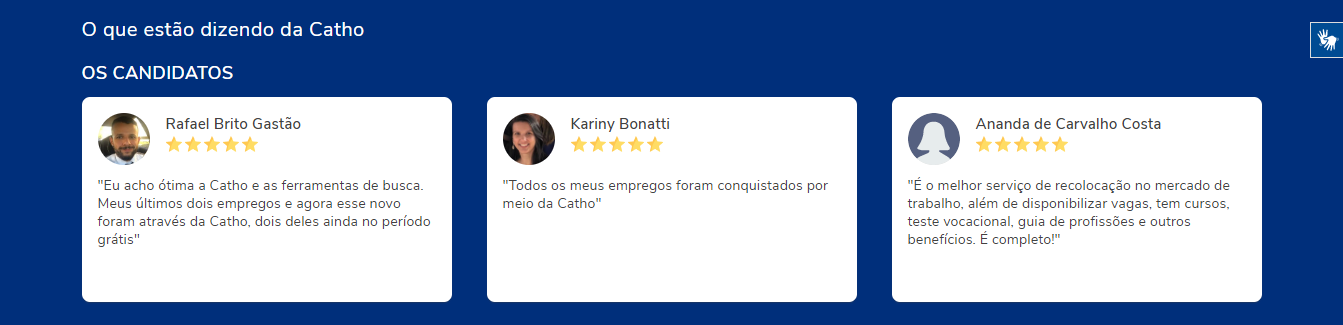
\includegraphics[width=400px, height=150px]{./images/cathoMobile1.png}
	\par {Autor(a): \cite{catho-3}}
\end{figure}

\newpage
\subsubsection{Estudo de Caso – GetNinjas}

É um app que traz facilidade para pessoas que buscam por profissionais, serviços ou até mesmo por clientes. Getninjas está disponível nas plataformas Android, (IOS) Iphone, assim como na WEB.

\begin{figure}[!h]
	\centering
	\caption{Pagina inicial}
	\includegraphics[width=150px, height=250px]{./images/getNinjasMobile2.jpeg}
	\par {Autor(a): \cite{get-ninjasMobilea}}
\end{figure}

Para utilizar o aplicativo é necessário que seja feito um cadastro do usuário. As pessoas que procuram por profissionais, conseguem contratar diaristas, cabelereiros, buffet, Dj, consultoria, entre outros. Getninjas possui diversas áreas na qual você consegue fazer uma busca por profissionais. O aplicativo fará uma busca e de acordo com a proximidade o mesmo traz a você até 3 profissionais das áreas em que busca, com isso eles entraram em contato para que possam passar o orçamento.

Geralmente é um pouco difícil achar algum profissional qualificado que faça o que está precisando. No aplicativo Getninjas além de conseguir fazer uma busca rápida sobre quais profissionais da área tem por perto, você consegue ver a avaliação do profissional, com isso você já está ciente se é um bom profissional ou não. Ao mesmo tempos que as pessoas procuram por profissionais bons, os profissionais autônomos e freelancers também tem dificuldade quando buscam por clientes e serviços, por isso a Getninjas ajuda tanto, pois foi criada com o objetivo de unir ambas as necessidades. Tem um marketplace que ajuda tanto encontrando profissionais para o serviço desejado quanto facilitando que você seja encontrado por clientes potenciais.

O aplicativo também serve para pessoas que desejam atrair clientes, é necessário preencher os campos com o serviço no qual será oferecido e as atividades da pessoa para que você consiga entrar em contato e passar o orçamento.

O cadastro para ambos os objetivos é bem rápido e prático. O aplicativo é grátis e você só paga pelo serviço que contratar. O aplicativo é uma boa opção tanto para quem busca profissionais, como também para quem está buscando por empregos. Não há um número de vagas e com isso qualquer um pode oferecer seus serviços.

\begin{figure}[!h]
	\centering
	\caption{Cadastro }
	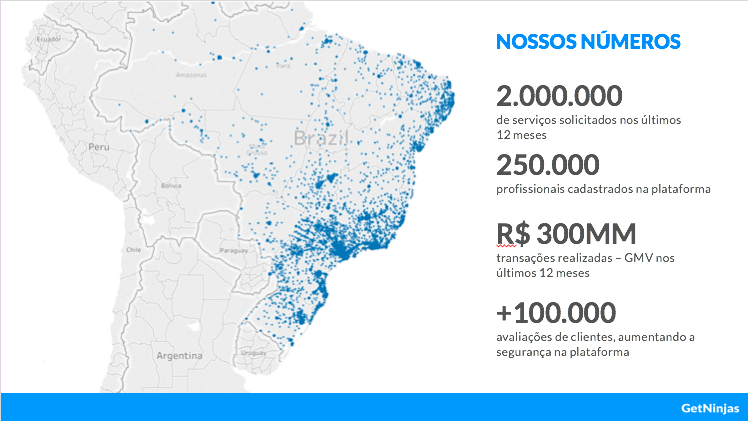
\includegraphics[width=150px, height=220px]{./images/getNinjasMobile.jpeg}
	\par {Autor(a): \cite{get-ninjasMobilea}}
\end{figure}

Para quem precisa de um serviço é necessário ter disposição de dois formulários. No primeiro você precisa especificar sobre o serviço desejado. No segundo, o endereço no qual o cliente quer que o trabalho seja realizado, e logo em seguida o aplicativo manda uma mensagem para o celular da pessoa com o código para confirmar o pedido.

\begin{figure}[!h]
	\centering
	\caption{Pesquisa de profissionais}
	\includegraphics[width=150px, height=180px]{./images/getNinjasMobile3.jpeg}
	\par {Autor(a): \cite{get-ninjasMobilea}}
\end{figure}
\newpage

Quando ocorre a confirmação o aplicativo avisa a todos os profissionais que se enquadram na descrição, levando em conta a distância. Os três primeiros que responderem ao chamado recebem os dados do cliente e entram em contato com o mesmo para que possam passar o orçamento. No fim o cliente escolhe o que for de sua preferência.

Para quem presta serviços, é necessário se cadastrar na plataforma, informando dados como qual o serviço que oferece, CEP e número de celular. Depois é preciso dar detalhes sobre as atividades e por fim criar um anúncio para se auto divulgar.

O anúncio é a porta de entrada do serviço, com isso o aplicativo incentiva os profissionais a explicarem bem detalhadamente quais suas qualidades e seus diferenciais. Após criar seu anúncio você preenche com o CPF ou CNPJ, endereço e confirma o cadastro com o código enviado. Por fim o profissional fica no aguardo do aplicativo sinalizá-lo quando tiver um pedido para entrar em contato com o cliente e passar seu orçamento.

O diferencial do Getninjas é o poder de escolha aos profissionais, que recebem pedidos conforme a distância, velocidade, entre outros. Além disso tem a possibilidade de facilitar o processo de pagamento via app, liberado com o pacote de créditos que são necessários para que os pedidos sejam liberados.

Com apenas 6 anos a startup conseguiu o lugar de maior classificado de serviços online do país, com uma média de duzentos e cinquenta mil profissionais cadastrados, além de que no último ano ela teve dois milhões de serviços solicitados gerando R\$ 300 Milhões em transações realizadas.

\begin{figure}[!h]
	\centering
	\caption{Pesquisa de campo}
	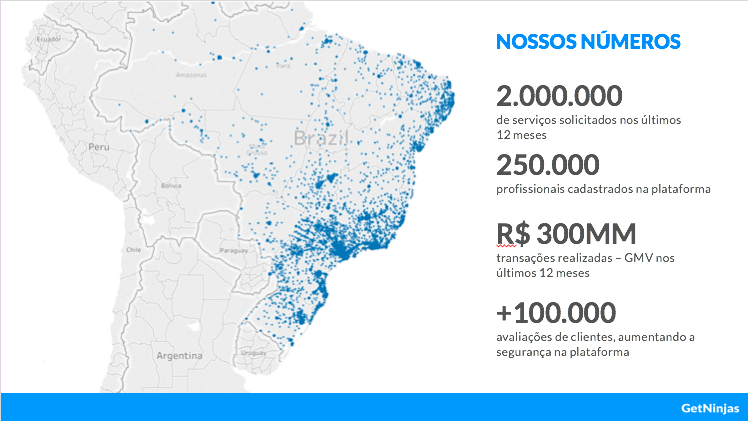
\includegraphics[width=300px, height=170px]{./images/getNinjasMobile.png}
	\par {Autor(a): \cite{get-ninjasMobile}}
\end{figure}
\newpage


